\section{Results}

Maximum of 1200 words.

The results describe in depth the actual, substantive results achieved, logically
following from the method used. Name the concrete artefact that (for the client) forms the end product of the delivered work. Indicate what type of artefact it is, for example a design, an architecture, a model or a software application. Then describe in depth the content of the artefact based on the (which?) requirements, the (which?) relevant insights from grounding and the (which?) relevant insights from
activities within the design cycle. Use illustrations where useful, this is very clarifying compared to texts in (long) paragraphs only. Where possible, also use lists and/or tables for readability.

% Code below is an example of how various things in LaTeX can be inserted, such as code snippets, tables, etc.

\subsection{Examples}

Inserting an image can be done as followS:

\begin{figure}[H]
    \centering
    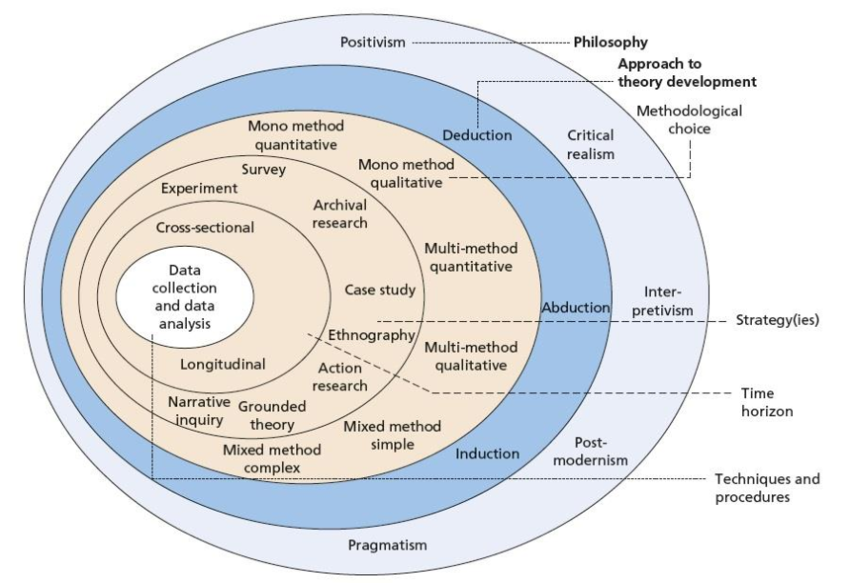
\includegraphics[width=.8\linewidth]{figures/Research-onion-4.png}
    \caption{The research onion (adopted from \cite{siti2020}). [for illustration purposes only, so remove from the EA].}
    \label{fig:onion}
\end{figure}

You may want to insert \texttt{Python} code snippets to show the design of your algorithm. We created a \texttt{Python} macro in the preamble that makes it easy to insert snippets of code. This environment takes two arguments \verb|\begin{python}(caption)(label)| where:
\begin{enumerate}
    \item \textit{caption} can be used to provide a description for this code listing
    \item \textit{label} can be used as an identifier to reference this listing in the text
\end{enumerate}

\noindent As an example, consider listing~\ref{lst:foo}.

\begin{python}{Important algorithm}{lst:foo}
def foo(x: int, y: float) -> str:
    z = x + y
    return "Hello " + z
\end{python}

\noindent There is also the option to write pseudo code in \LaTeX. See the following example in algorithm~\ref{alg:wfc}. 

\begin{algorithm}[H]
\caption{Simplified version of the Wave Function Collapse algorithm}\label{alg:wfc}
\hspace*{\algorithmicindent} \textbf{Input}: Sample image $img$;\\
\hspace*{\algorithmicindent} \textbf{Output}: Rendered output image
\begin{algorithmic}[1]
\Function{WFC}{$img$}
\State patterns := ExtractFromSample($img$);
\State ConstructIndex(patterns);
\State InitialiseGrid(patterns);
\Repeat 
    \State $p$ := Observe();
    \If{$p = null$}
        \State \textbf{break};
    \EndIf
    \State Collapse($p$);
    \State Propagate();
\Until{all variables are observed}
\State \Return ObservationsToOutput(); 
\EndFunction
\end{algorithmic}
\end{algorithm}

\noindent Often, you evaluate your artifacts quantitatively, elicit requirements from stakeholders, or may aggregate guidelines from the contemporary literature. In these cases, it can be useful to display these results in a table. See table~\ref{tab:example1},~\ref{tab:example2}, and~\ref{tab:example3} for various table examples. 

\def\arraystretch{1.5}%  1 is the default, change whatever you need
\begin{table}[H]
    \centering
    \caption{Confusion matrix for two classes.}
    \label{tab:example1}
    \vspace{-2mm}
    \begin{tabular}{|c|c|c|c|}
    \hline
        & \multicolumn{3}{c|}{\textit{Predicted class}} \\\hline
        \textit{True class} & \textbf{Positive} & \textbf{Negative} & \textit{Total} \\\hline
        \textbf{Positive} & $tp$: true positive & $fn$: false negative & $p$\\\hline
        \textbf{Negative} & $fp$: false positive & $tn$: true negative & $n$\\\hline
        \textit{Total} & $p'$ & $n'$ & $N$\\\hline
    \end{tabular}
\end{table}

\begin{table}[H]
    \centering
    \caption{Evaluation results of the selected hypothesis classes over 98 repetitions of training/testing splits for both the baseline as well as the difference datasets. Mean AUC and cross-entropy loss are reported. }\label{tab:example2}
    \vspace{-2mm}
    \makebox[\linewidth]{
        \begin{tabular}{l|cc|cc}
            \toprule
                \multicolumn{1}{c}{} & \multicolumn{2}{c}{\textbf{Baseline}} & \multicolumn{2}{c}{\textbf{Difference}} \\ 
            \cmidrule(rl){2-3} \cmidrule(rl){4-5}
                \textbf{Model} & \emph{AUC} & \emph{Cross-entropy} & \emph{AUC} & \emph{Cross-entropy} \\
            \midrule
                Random Forest & $0.605 \pm 0.010$ & $12.227 \pm 0.332$ & $0.609 \pm 0.012$ & $12.281 \pm 0.377$ \\
                XGBoost Classifier & $0.617 \pm 0.014$ & $12.474 \pm 0.456$ & $0.612 \pm 0.012$ & $12.314 \pm 0.394$ \\
                Support Vector Machine & $0.560 \pm 0.017$ & $15.220 \pm 0.631$ & $0.511 \pm 0.007$ & $14.453 \pm 0.242$ \\
                Multi-Layer Perceptron & $\bm{0.622 \pm 0.012}$ & $\bm{12.096 \pm 0.423}$ & $\bm{0.618 \pm 0.011}$ & $\bm{12.155 \pm 0.355}$ \\
            \bottomrule
        \end{tabular}
    }
\end{table}

\begin{table}[H]
    \centering
    \caption{Hyperparameter search space for the Random Forest classifier.}\label{tab:example3}
    \vspace{-2mm}
    \makebox[\linewidth]{
        \begin{tabularx}{\textwidth}
        % {lXr}
         {
            >{\raggedright\arraybackslash}p{.24\textwidth}
            >{\raggedright\arraybackslash}p{.4\textwidth}
            X
        }
            \toprule
                \textbf{Parameter} & \textbf{Description} & \textbf{Values} \\
            \midrule
                \texttt{n\_estimators} & Number of decision tree estimators. & $[50, 5000]$ with steps of 50.\\
                \texttt{min\_samples\_leaf} & Minimum number of instances required at a leaf node. & $[5, 50]$ with steps of 5.\\
                \texttt{max\_depth} & Maximum depth of the decision trees. & $[4, 24]$\\
                \texttt{criterion} & Function to measure quality of a split. & \texttt{'gini'} or \texttt{'entropy'}\\
                \texttt{max\_features} & For $d$ features, it is the $k<d$-features to consider when looking for the best split. & $\sqrt{d}$ or $\log_2(d)$, or fractions of $d$: 0.1, 0.3, 0.5, 0.7, 0.9. \\
                \texttt{bootstrap} & Whether bootstrap samples are used when building trees. & \texttt{True} or \texttt{False}\\
            \bottomrule
        \end{tabularx}
    }
\end{table}